% Chapter Template

\chapter{Mapping and Scheduling} % Main chapter title

\label{c:sched} % Change X to a consecutive number; for referencing this chapter elsewhere, use \ref{ChapterX}

%----------------------------------------------------------------------------------------
%	SECTION 1
%----------------------------------------------------------------------------------------

\section{Schedulability Analysis}

\addfigure{0.6}{modes.pdf}{The 4 modes of operation in MCFTS analysis}{f:modes}

\addfigure{0.55}{ftm.pdf}{The 4 fault tolerance mechanisms supported by the proposed MCFTS analysis}{f:ftm}

\begin{equation}
R_i^{(LO)}= C_i(LO)+\sum_{j \in hp(i)}\Big\lceil\frac{R_i^{(LO)}}{T_j}\Big\rceil \cdot C_j(LO)
\label{eq:lomode}
\end{equation}

\begin{equation}\label{eq:tfmode}
\begin{aligned}
R_i^{(TF)} & = n_i(TF) \cdot C_i(LO)
+\sum_{j \in hpC(TF,i)}\Big\lceil\frac{R_i^{(TF)}}{T_j}\Big\rceil \cdot n_j(TF) \cdot C_j(LO) \\
&  +\sum_{k \in hp(i)-hpC(TF,i)}\Big\lceil\frac{R_i^{(LO)}}{T_k}\Big\rceil \cdot C_k(LO)
\end{aligned}
\end{equation}

\begin{equation}\label{eq:ovmode}
\begin{aligned}
R_i^{(OV)} &  = C_i(L_i)+\sum_{j \in hpC(OV,i)}\Big\lceil\frac{R_i^{(OV)}}{T_j}\Big\rceil \cdot C_j(L_j) 
 +\sum_{k \in hp(i)-hpC(OV,i)}\Big\lceil\frac{R_i^{(LO)}}{T_k}\Big\rceil \cdot C_k(LO)
\end{aligned}
\end{equation}


\begin{equation}\label{eq:hitfmode}
\begin{aligned}
R_i^{(HIa)} & = n_i(HI) \cdot C_i(L_i) 
  +\sum_{j \in hpC(HI,i)}\Big\lceil\frac{R_i^{(HIa)}}{T_j}\Big\rceil \cdot n_j(HI) \cdot C_j(L_j) \\
&  +\sum_{k \in hpC(TF,i)-hpC(HI,i)}\Big\lceil\frac{R_i^{(TF)}}{T_k}\Big\rceil \cdot C_k(LO)
  +\sum_{l \in hp(i)-hpC(TF,i)}\Big\lceil\frac{R_i^{(LO)}}{T_l}\Big\rceil \cdot C_l(LO)
\end{aligned}
\end{equation}

\begin{equation}\label{eq:hiovmode}
\begin{aligned}
R_i^{(HIb)} & = n_i(HI) \cdot C_i(L_i) 
  +\sum_{j \in hpC(HI,i)}\Big\lceil\frac{R_i^{(HIb)}}{T_j}\Big\rceil \cdot n_j(HI) \cdot C_j(L_j) \\
&  +\sum_{k \in hpC(OV,i)-hpC(HI,i)}\Big\lceil\frac{R_i^{(OV)}}{T_k}\Big\rceil \cdot C_k(LO)
  +\sum_{l \in hp(i)-hpC(OV,i)}\Big\lceil\frac{R_i^{(LO)}}{T_l}\Big\rceil \cdot C_l(LO)
\end{aligned}
\end{equation}



lockstep:
\begin{itemize}
  \item $N=<1,2,1,2>$
  \item Task set does not change.
  \item No constraints are required because there are no replicas.
\end{itemize}

dmr:
\begin{itemize}
  \item One replica
  \item $N=<1,2,1,2>$
  \item For each task $\tau_i$ with replica $\tau_j$, constraint is generated that processor $\pi_i \ne \pi_j$
  \item In example: $\pi_1 \ne \pi_{1.1}$
\end{itemize}
\begin{table}
\centering
\caption{Example task set}
\begin{tabular}{@{}l|cccc@{}}
\toprule
		& C(LO) & C(HI) & T=D & L 	 \\\bottomrule
$\tau_1$ & 5 & 10 & 25 & HI  \\
$\tau_2$ & 5 & - & 20 & LO  \\
$\tau_3$ & 2 & - & 8 & LO  \\
\end{tabular}
\end{table}


\begin{table}
\centering
\caption{Updated task set}
\begin{tabular}{@{}l|cccc@{}}
\toprule
		& C(LO) & C(HI) & T=D & L	 \\\bottomrule
$\tau_1$ & 5 & 10 & 25 & HI  \\
$\tau_{1.1}$ & 5 & 10 & 25 & HI  \\
$\tau_2$ & 5 & - & 20 & LO  \\
$\tau_3$ & 2 & - & 8 & LO  \\
\end{tabular}
\end{table}


tmr:
\begin{itemize}
  \item Two replicas
  \item $N=<1,1,1,1>$
  \item For each task $\tau_i$ with replica $\tau_j$, constraint is generated that processor $\pi_i \ne \pi_j$
  \item In example: $\pi_1 \ne \pi_{1.1} \ne \pi_{1.2}$
\end{itemize}
\begin{table}
\centering
\caption{Example task set}
\begin{tabular}{@{}l|cccc@{}}
\toprule
		& C(LO) & C(HI) & T=D & L 	 \\\bottomrule
$\tau_1$ & 5 & 10 & 25 & HI  \\
$\tau_2$ & 5 & - & 20 & LO  \\
\end{tabular}
\end{table}

\begin{table}
\centering
\caption{Updated task set}
\begin{tabular}{@{}l|cccc@{}}
\toprule
		& C(LO) & C(HI) & T=D & L	 \\\bottomrule
$\tau_1$ & 5 & 10 & 25 & HI  \\
$\tau_{1.1}$ & 5 & 10 & 25 & HI  \\
$\tau_{1.2}$ & 5 & 10 & 25 & HI  \\
$\tau_2$ & 5 & - & 20 & LO  \\
\end{tabular}
\end{table}

passive replication:
\begin{itemize}
  \item Two replicas.
  \item $N=<1,1,1,1>$ for the original and one replica, $N=<0,1,0,1>$ for the other.
  \item In example: $\pi_1 \ne \pi_{1.1}$, $\pi_{1.2}$ can execute on any core.
\end{itemize}

\begin{table}
\centering
\caption{Example task set}
\begin{tabular}{@{}l|cccc@{}}
\toprule
		& C(LO) & C(HI) & T=D & L 	 \\\bottomrule
$\tau_1$ & 5 & 10 & 25 & HI  \\
$\tau_2$ & 5 & - & 20 & LO  \\
\end{tabular}
\end{table}

\begin{table}
\centering
\caption{Updated task set}
\begin{tabular}{@{}l|cccc@{}}
\toprule
		& C(LO) & C(HI) & T=D & L	 \\\bottomrule
$\tau_1$ & 5 & 10 & 25 & HI  \\
$\tau_{1.1}$ & 5 & 10 & 25 & HI  \\
$\tau_{1.2}$ & 5 & 10 & 25 & HI  \\
$\tau_2$ & 5 & - & 20 & LO  \\
\end{tabular}
\end{table}


\subsection{Design Space Exploration}

The initial scheduling algorithm will be taken from Bolchini and  Miele \cite{bolchini2013reliability}. A genetic algorithm (GA) is used to explore the design space. The general details that follow on genetic algorithms are based on the overview in \cite{geatbx}.

Figure \ref{f:ga_ov} shows an overview of how to implement a genetic algorithm. There are two stages of GA in the given process. First tasks must be organized into groups of tasks, and each group of tasks must be assigned a fault detection technique or fault tolerance technique. DMR Fingerprinting is an example of a detection mechanism. This work will remain agnostic about the method of implementation of fault tolerance. We assume that appropriate hardening measures are applied to a single core.
 
\begin{figure}[h]
\centering
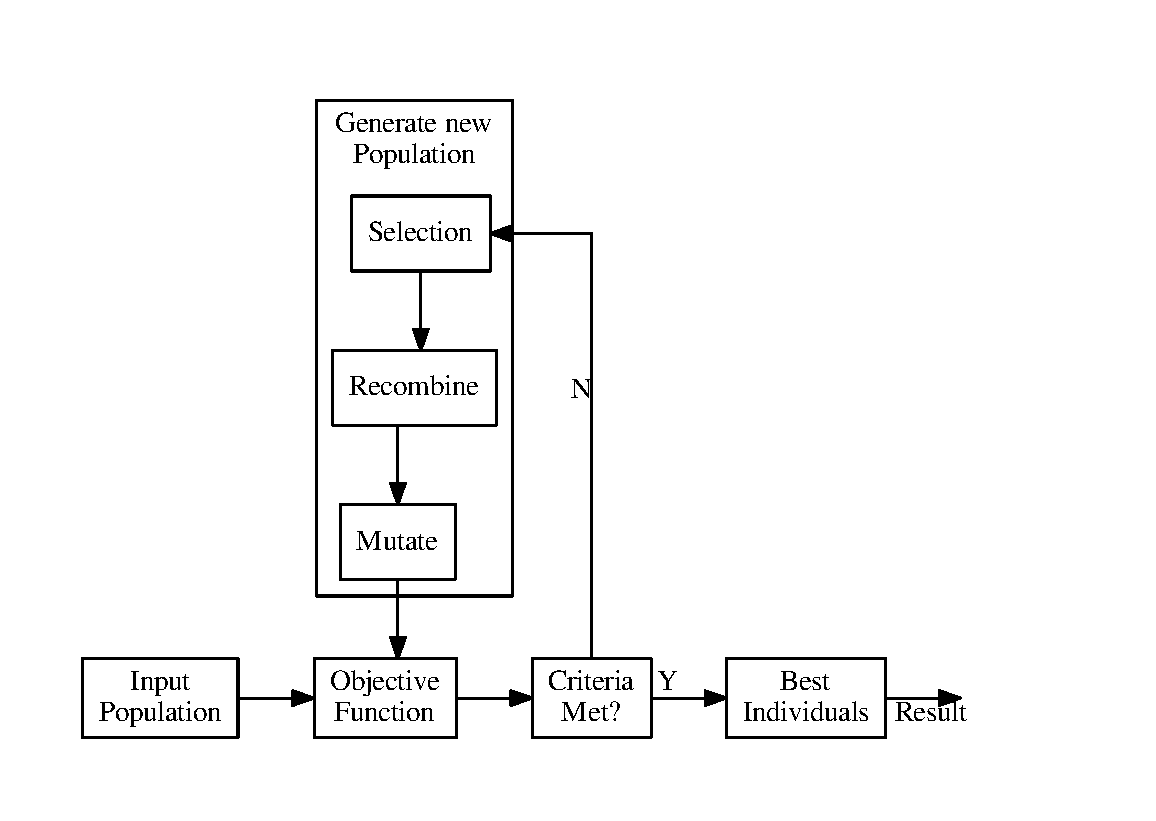
\includegraphics[width=12cm]{ga_ov}
\caption{The basic structure of a genetic algorithm \cite{geatbx}.}
\label{f:ga_ov}
\end{figure}

Once a population of various groupings and associated fault-handling mechanisms has been generated it is necessary to test their fitness. This must be done by generating a system schedule for each member of the population. 

The generation of the schedule is itself done with a second round of GA. Each task is assigned to an appropriate core based on the fault-handling requirements of its group. The group adopts the most stringent requirements of any of its members. Various mappings are generated as the GA population. Then it is necessary to order the tasks on each core. This is complicated by the fact that there may be inter-core data dependencies. For now, we will neglect the overhead associated with data transfer between cores.

The implementation details of the genetic algorithm will be adopted from \cite{bolchini2013reliability}. Tournament selection and single-point crossover operator recombination will be used. Mutations will be applied randomly. There are four mutations at the task level: change the group of a task, split a group in two, join two groups, or change the fault-management technique applied to a group. The mutation for the mapping phase consists of switching a task to another processor that can meet the assigned fault-management requirements.

Tournament selection means choosing a subset of the population and selecting the most fit member. This is repeated as many times as necessary. Single-point crossover cuts two parent chromosomes into two pieces and then exchanges the second substrings between the chromosomes. 

The initial parameters for the GA will be the ones suggested in \cite{bolchini2010multi}. The crossover rate is 80\%, the mutation rate is 10\%. The program will run for 30 generations. The population size will be between one and two thousand.

The JGAP library \cite{jgap} is used to implement the genetic algorithm. 



